\chapter{Implementation}
\begin{figure} \label{fig:filterblock}
	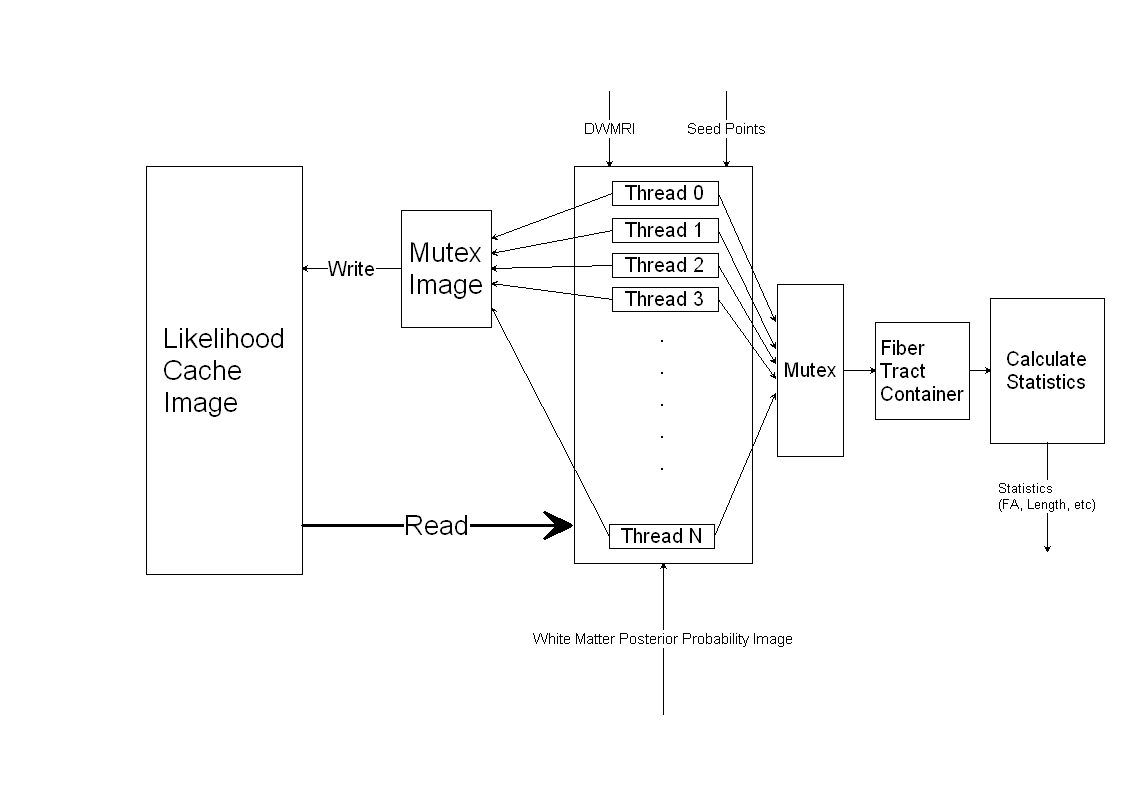
\includegraphics[width=0.5\linewidth]{filterblock}
	\caption{A block diagram of the filter showing its shared likelihood cache and multithreaded architecture.}
\end{figure}
In implementing the system a few concerns were addressed.  First, we wanted the system to be accessible to the largest audience as possible.  To enable this, the algorithm was implemented as an extension to the ITK toolkit.  The ITK toolkit is a collection of image processing and statistical analysis algorithms that are relevant to biomedical imaging applications.  Additionally, the ITK toolkit is opensource software, which allows other researchers to look at how the algorithm was implemented in order to make further modifications.  Including the algorithm in the ITK package would instantly provide a large existing research community with access ot the algorithm.  Additionally, a GUI module was created for the 3D Slicer medical visualization program to provide which enable researchers using this environment easy access to the algorithm via an intuitive visual interface, while the ITK module can be used as a stand alone command line program suitable for noninteractive processing of large numbers of data sets.  Choosing to implement the algorithm in tools with an already established audience already familar with these environments would faciliate adoption of the algorithm in clinical studies.

The second major concern lies in the potentially long computational time of the algorithm.  Since this algorithm is a monte carlo class algorithm which is sampling a high dimensional parameter space, it may take many samples the posterior distribution of these parameters converges.  The run time order of growth these algorithms grows exponentially with the number of paramters.  Since a fiber tract is characterized by a sequence of segment orientations, each of the orientations is a parameter of the fiber tract.  These tracts vary in length but on average they consist of approximately 60 segments and hence 60 parameters.  Sampling in such a high dimensional space may require many sample before the distributions converges on the true distribution.  We address these concerns by implementing the algorithm in a multithreaded manner and in our use of a shared likelihood distribution cache between these threads.  The multithreaded design reduces computation time approximately linearly with the number of processors and the use of a likelihood cache, while not reducing the order of growth of the algorithm, reduces the incremental cost of generating each additional tract.

Although the itk framework contains a framework for implementing algorithms in a multithreaded manner, this framework is not suitable for the stochastic tractography algorithm.  The itk multithreading framework assumes that the output region can be divided into disjoint sections with each thread working exclusively on their own section of the output image.  This design prevents the threads from concurrently writing to the same region which may cause unexpected results.  However, since the stochastic tractography algorithm generates tracts that which may span the entire output image, this exclusive division of the output region is not possible.  Instead each thread of the itk module contains an essentially independent instance of the probabilistic tractography algorithm. Each thread allocates memory for the tract that they are generating.  Once the tract has been completed, the thread stores a pointer to the completed tract in a shared tract pointer vector.  The tract pointer vector is protected by a mutex, which serializes write operations so that only one thread can store its completed tract in the vector at a time.  Once enough samples have been accumulated, the tracts can be transferred to the output image to create a connectivity map or other statistics can be computed on them.  In essence, we divide the process into two sections, a multithreaded portion that samples the tracts and a single threaded portion which accumulates the tracts and calculates relevant statistics on them.

The most computationally expensive part of the algorithm is the calculation of the likelihood distribution.  The algorithm must compute probabilites for over 2000 possible fiber orientations in a voxel.  Fortunately, this likelihood distribution is a deterministic function of the diffusion observations within that voxel.  This allows us to cache the likelihood distribution if the algorithm were to encounter it later.  Additionally, in anisotropic regions of the brain, the sampled threads are expected to have some coorellation due to the underlying diffuision data.  This causes many of the sampled tracts to visit the same voxels many times.  

The cache is designed as an itk image whose voxels are dynamic array types.  It was implemented as an image to take advantage of itk's fast access of objects indexed by image coordinates.  Initially every voxel in the likelihood cache image is initiated to a zero length array.  When the algorithm encounters a voxel, it first checks to see if the likelihood cache contains this voxel by checking if the associated array is zero length.  If the array is zero length, this means the voxel has never been visited and it resizes the array associated with the voxel of interest inside the likelihood cache, computes the likelihood distribution associated with this voxel and stores it inside of this newly resized array.

An additional difficult is caused by using a shared likelihood cache multiple concurrent threads.  Simultaneous writes to the cache will caused unexpected behaviour and there is also the possibility of a thread reading incomplete cache information that is simultaneously being written by another thread.  One possible solution is to ensure that only one thread can read or write to the likelihood cache at a time.  This is easily implemented by using a mutex or mutually exclusive lock.  A mutex is an object that serves as lock.  A thread will wait until a mutex if unlocked before it proceeds to the next section of code.  Inside this section, which is called the critical section, the thread locks the mutex to ensure that no other threads attempt any operations on the shared data before the thread which currently owns the lock finishes its operations.  All other threads must wait and idle while the thread which owns the lock finishes it operations.  Since the algorithm must access the likelihood cache very often, this results in a situation where many threads are waiting for other threads to finish accessing the likelihood cache.  The bottleneck is now the serialized access to the likelihood cache which in the worse case would result in performance that is only slightly better than the single threaded version.

These access collisions to the likelihood cache can be reduced if we increase the resolution of the lock.  In other words, instead of using one large lock for the entire likelihood cache image, we use a lock for each voxel.  The probability of two threads accessing the same voxel concurrently is much less than the probability that two threads access any part of the likelihood cache image.  These per voxel locks are conveniently constructed using an itk image whose voxel data type is a mutex.  Similar to the likelihood cache, this collection of mutexes are indexed by coordinates which correspond to the coordinates of the voxels in the DWI input data.  Again, access to the mutex image is fast thanks to ITK's optimized access operators for data types indexed by coordinates.  The only cost to using this high resolution mutex image is the additional memory required to store these mutexes.  However, since a mutex is essential a boolean variable, it is a very modest cost for a large increase in performance.  The mutex image allows different voxels in the likelihood cache image to be written to simultaneously, increaseing the rate at which the likelihood cache is filled.  In the ideal case where collisions are very unlikely to occur, such as tracking in a highly isotropic region, where sampled paths have very low correlation, this design will allow the rate of tract sampling to scale linearly with the number of threads, provided each thread runs on its own processor.  It may also be advantageous to run more than multiple threads on a uniprocessor computer since it will increase the rate at which the likelihood cache is filled since the probability multiple the threads encountering an unvisited voxel is higher than a single thread.
%block diagram

\section{Optimizations}
The paramters of the tensor model is computed for each voxel encountered by the algorithm using a WLS estimate.  In computing this WLS estimate, we must first estimate the weights.  These weights are found by calculating a LS estimate of the true intensities of each voxel.  Since the same $A$ matrix is used for each voxel in the computation of these weights a common optimization is to orthogonalize the $A$ matrix by computing its QR decomposition.  While computationally expensive, this computation is performed once and is used to calculate the weights for every encountered voxel.

\section{3D Slicer Module}
%slicer3 module
%include figure
The 3D Slicer visualization program is extensively used by some clinical groups, such as the BWH to visualize and analyze data.  To encourage the algorithm's adoption in clinical studies an interactive GUI module for the 3D Slicer medical image visualization program was created which interfaces with the ITK module.

The module was implemented using the command line module interface provided by the 3D Slicer environment.  This interface greatly eased the adaption of the command line itk module into a module that could interface with 3D Slicer.  The interface for the module was described using an xml file.  This file is processed by a program provided with 3D Slicer to produce a C++ file that is included with the ITK command line module.  This C++ file provides functions which parse command line parameters and allows the module to interface with the 3D Slicer environment.  As an added benefit, the ITK module can still be run as a stand alone program to batch process large numbers of subjects noninteractively.

%inputs
%outputs
%parameters

